%% LyX 2.4.4 created this file.  For more info, see https://www.lyx.org/.
%% Do not edit unless you really know what you are doing.
\documentclass[english,t]{beamer}
\usepackage{mathptmx}
\usepackage[T1]{fontenc}
\usepackage[latin9]{inputenc}
\usepackage{amssymb}
\usepackage{cancel}

\makeatletter

%%%%%%%%%%%%%%%%%%%%%%%%%%%%%% LyX specific LaTeX commands.
%% Because html converters don't know tabularnewline
\providecommand{\tabularnewline}{\\}

%%%%%%%%%%%%%%%%%%%%%%%%%%%%%% Textclass specific LaTeX commands.
% this default might be overridden by plain title style
\newcommand\makebeamertitle{\frame{\maketitle}}%
% (ERT) argument for the TOC
\AtBeginDocument{%
  \let\origtableofcontents=\tableofcontents
  \def\tableofcontents{\@ifnextchar[{\origtableofcontents}{\gobbletableofcontents}}
  \def\gobbletableofcontents#1{\origtableofcontents}
}

%%%%%%%%%%%%%%%%%%%%%%%%%%%%%% User specified LaTeX commands.
\usetheme{Warsaw}
% or ...

\setbeamercovered{transparent}
% or whatever (possibly just delete it)
\setbeamercovered{invisible} %makes overlays invisible

%gets rid of navigation symbols
\setbeamertemplate{navigation symbols}{}

%\usepackage{hyperref}
%\usepackage[usenames,dvipsnames,table]{xcolor} %adds additional color options
\definecolor{links}{HTML}{2A1B81}
%\hypersetup{colorlinks,linkcolor=blue,urlcolor=links}

\usepackage{multicol}

\usepackage{tikz}
\usetikzlibrary{calc}
\usetikzlibrary{plotmarks}
\usetikzlibrary{shapes}
\usepackage{pgfplots}
\pgfplotsset{compat=newest}

\usepackage{forest} %%for tree diagram

\usepackage{calc}
\usepackage[nomessages]{fp}

%\usepackage{advdate}    % Advancing/saving dates
\usepackage{datetime}   % Dates formatting
%\usepackage{datenumber} % Counters for dates

\usepackage[super]{nth}

\usepackage{etex}

\usepackage{fancybox}

%%table colors
%\usepackage[table]{xcolor}
\usepackage{colortbl}

\usepackage[outline]{contour}  %allows text halos
\contourlength{1pt} %sets halo width
%%example: \node at (0.75,0.5) {\contour{white}{\Large Text!}};
%%example:  \node [fill=white,inner sep=1pt] at (2.25,0.5) {\Large 			Text!};
%%example:  \node [fill=white,rounded corners=2pt,inner sep=1pt] at 			(3.75,0.5) {\Large Text!};

%%%%%%%%%%%%%%%%%%%%%%%%%%%
\def\formatdateny{\csname noyear\languagename\expandafter\endcsname\formatdate}
\def\noyearenglish#1, \the\@year{#1}
\let\noyearamerican\noyearenglish
\let\noyearbritish\noyearenglish

%%allows uncover with forest diagrams
\tikzset{
    invisible/.style={opacity=0,text opacity=0},
    visible on/.style={alt=#1{}{invisible}},
    alt/.code args={<#1>#2#3}{%
      \alt<#1>{\pgfkeysalso{#2}}{\pgfkeysalso{#3}} % \pgfkeysalso doesn't change the path
    },
}
\forestset{
  visible on/.style={
    for tree={
      /tikz/visible on={#1},
      edge={/tikz/visible on={#1}}}}}

%%%redefines column alignment to match vertically
%\define@key{beamerframe}{t}[true]{% top
  %\beamer@frametopskip=.2cm plus .5\paperheight\relax%
  %\beamer@framebottomskip=0pt plus 1fill\relax%
 % \beamer@frametopskipautobreak=\beamer@frametopskip\relax%
  %\beamer@framebottomskipautobreak=\beamer@framebottomskip\relax%
  %\def\beamer@initfirstlineunskip{}%
%}

%%provides pdf with 4 slides per page; don't forget to add 'handout' to remove overlays
%\usepackage{pgfpages}
%\pgfpagesuselayout{4 on 1}[a4paper, landscape, border shrink=7mm]
%\pgfpageslogicalpageoptions{1}{border code=\pgfusepath{stroke}}
%\pgfpageslogicalpageoptions{2}{border code=\pgfusepath{stroke}}
%\pgfpageslogicalpageoptions{3}{border code=\pgfusepath{stroke}}
%\pgfpageslogicalpageoptions{4}{border code=\pgfusepath{stroke}}
%%%Don't forget to add 'handout'

\makeatother

\usepackage{babel}
\begin{document}
\newcommand{\xmax}{2000}
\newcommand{\xmin}{0}
\newcommand{\xstep}{0} %must be xmin+n
\newcommand{\ymax}{500}
\newcommand{\ymin}{0}
\newcommand{\ystep}{0} %must be ymin+n

\newcounter{countEx} \setcounter{countEx}{0}
\newcounter{countProb} \setcounter{countProb}{0}
\resetcounteronoverlays{countEx} \resetcounteronoverlays{countProb}

\newcommand{\ex}[3]{
	\addtocounter{countEx}{1}
	\only<#1-#2>{\begin{exampleblock} {Example \chNum.\secNum.\arabic{countEx}.} #3	\end{exampleblock}}
}

\newcommand{\prob}[4]{
	\addtocounter{countProb}{1}
	\only<#1-#2>{\begin{exampleblock} {Problem  \chNum.\secNum.\arabic{countProb}.\,#3} #4	\end{exampleblock}}
}

\newcommand{\yline}[4]{
	(#2 - #4)/(#1 - #3)*(x - #1) + #2
}

\beamerdefaultoverlayspecification{<+->}

%%%%Chapter and Section numbers%%%%%
\newcommand{\chNum}{1}
\newcommand{\secNum}{4}
\newcommand{\secTitle}{Analyzing Arguments}
\date{\formatdate{24}{9}{2014} \& \formatdate{26}{9}{2014}}

\title[Section \chNum.\secNum: \secTitle]{Section \chNum.\secNum: \secTitle}

\subtitle{Finite Mathematics~~MTH 107~~Fall 2014}

\author{Dr.\,James Ashe}

\titlegraphic{\includegraphics[height=2.75cm]{/home/jim/JamesAshe/MHU/images/MarsHilUniversityLogo-Virtical.png}}

\institute{Mars Hill University}

\makebeamertitle 

%%True false command
\newcommand{\T}{\textcolor{green}{\contour{black}{T}}}
\newcommand{\F}{\textcolor{red}{\contour{black}{F}}}
\newcommand{\uT}[2]{\uncover<#1-#2>{\T}}
\newcommand{\uF}[2]{\uncover<#1-#2>{\F}}

%tkiz ball item 
\newcommand*\circled[1]{\tikz[baseline=(char.base)]
	{\node[circle,ball color=green!50!black!100, shade,   color=white,inner sep=1.2pt] (char) {\tiny #1};
	}
}
\begin{frame}{Recall: Valid/Invalid Arguments}

\vspace{-.5cm}
\begin{columns}


\column{5.5cm}
\begin{block}{Invalid Argument}
A deductive argument is \emph{invalid} if the premises are met, but
the conclusion does \emph{not necessarily} follow.

\begin{itemize}
\item <2->Using a Venn diagram.
\end{itemize}
\end{block}
\only<3-7>{
\begin{exampleblock}{Example}

\begin{enumerate}
\item []<3->If he is president he is a man. 
\item []<5->He is a man.
\item []<6->Therefore, he is a president.
\end{enumerate}
\end{exampleblock}
}

\only<8->{
\begin{exampleblock}{Example}

\begin{enumerate}
\item []<8->If he is president he is a man..
\item []<9->He is a president.
\item <10->[]Therefore, he is a man.
\end{enumerate}
\end{exampleblock}
}

\column{5.5cm}

\only<4>{%%%%little circle in big%%%%%
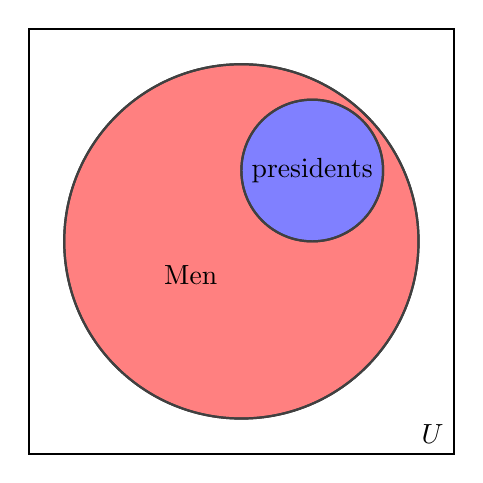
\begin{tikzpicture}[scale=.9]
	\def\circleA{(1,-1) circle (2.5)} %A
	\def\circleB{(0:2) circle (1)} %B

	\colorlet{circle edgeA}{black!75} 
	\colorlet{circle areaA}{red!50}
	\colorlet{circle edgeB}{black!75} 
	\colorlet{circle areaB}{blue!50}

	\tikzset{
		filledA/.style={fill=circle areaA, draw=circle edgeA, thick},
		filledB/.style={fill=circle areaB, draw=circle edgeB, thick},
		outlineA/.style={draw=circle edgeA, thick},
		outlineB/.style={draw=circle edgeB, thick},
	}

	\begin{scope}[fill opacity=1.0]         
			\fill[filledA] \circleA;
			\fill[filledB] \circleB;    
	\end{scope}

	\draw[outlineA] \circleA node[below left= 5pt] {Men}; 
	\draw[outlineB] \circleB node {presidents}; 
	%\node[anchor=south] at (current bounding box.north) {$A \cup B$}; 
	\draw[thick] (-2,-4) rectangle (4,2) node[anchor=south east] at (current bounding box.south east) {$U$};
	%\draw \circleA node[below=30pt,right=0pt] {\footnotesize{\emph{Dr.\,Ashe}}};
\end{tikzpicture} }\only<5-7>{%%%%little circle in big%%%%%
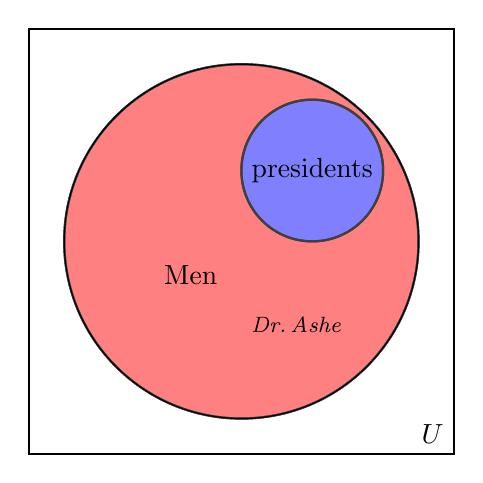
\begin{tikzpicture}[scale=.9]
	\def\circleA{(1,-1) circle (2.5)} %A
	\def\circleB{(0:2) circle (1)} %B

	\colorlet{circle edgeA}{black!75} 
	\colorlet{circle areaA}{red!50}
	\colorlet{circle edgeB}{black!75} 
	\colorlet{circle areaB}{blue!50}

	\tikzset{
		filledA/.style={fill=circle areaA, draw=circle edgeA, thick},
		filledB/.style={fill=circle areaB, draw=circle edgeB, thick},
		outlineA/.style={draw=circle edgeA, thick},
		outlineB/.style={draw=circle edgeB, thick},
	}

	\begin{scope}[fill opacity=1.0]         
			\fill[filledA] \circleA;
			\fill[filledB] \circleB;    
	\end{scope}

	\draw[outlineA] \circleA node[below left= 5pt] {Men}; 
	\draw[outlineB] \circleB node {presidents}; 
	%\node[anchor=south] at (current bounding box.north) {$A \cup B$}; 
	\draw[thick] (-2,-4) rectangle (4,2) node[anchor=south east] at (current bounding box.south east) {$U$};
	\draw \circleA node[below=30pt,right=0pt] {\footnotesize{\emph{Dr.\,Ashe}}};
\end{tikzpicture} }

\only<8>{%%%%little circle in big%%%%%
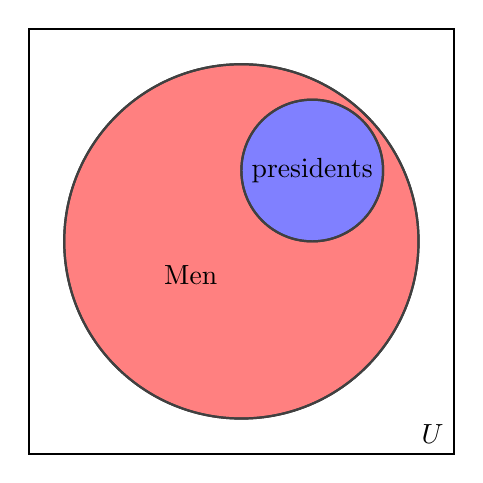
\begin{tikzpicture}[scale=.9]
	\def\circleA{(1,-1) circle (2.5)} %A
	\def\circleB{(0:2) circle (1)} %B

	\colorlet{circle edgeA}{black!75} 
	\colorlet{circle areaA}{red!50}
	\colorlet{circle edgeB}{black!75} 
	\colorlet{circle areaB}{blue!50}

	\tikzset{
		filledA/.style={fill=circle areaA, draw=circle edgeA, thick},
		filledB/.style={fill=circle areaB, draw=circle edgeB, thick},
		outlineA/.style={draw=circle edgeA, thick},
		outlineB/.style={draw=circle edgeB, thick},
	}

	\begin{scope}[fill opacity=1.0]         
			\fill[filledA] \circleA;
			\fill[filledB] \circleB;    
	\end{scope}

	\draw[outlineA] \circleA node[below left= 5pt] {Men}; 
	\draw[outlineB] \circleB node {presidents}; 
	%\node[anchor=south] at (current bounding box.north) {$A \cup B$}; 
	\draw[thick] (-2,-4) rectangle (4,2) node[anchor=south east] at (current bounding box.south east) {$U$};
	%\draw \circleA node[below=30pt,right=0pt] {\footnotesize{\emph{Dr.\,Ashe}}};
\end{tikzpicture} }\only<9->{%%%%little circle in big%%%%%
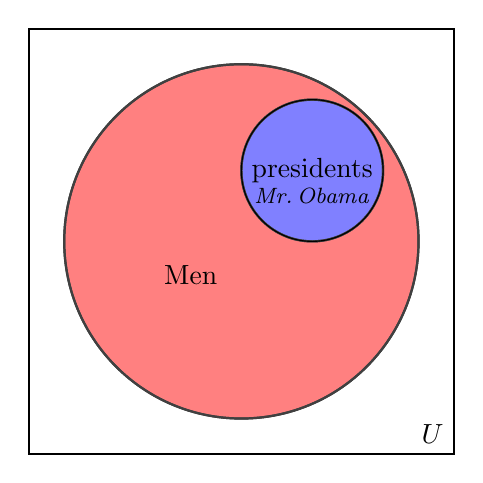
\begin{tikzpicture}[scale=.9]
	\def\circleA{(1,-1) circle (2.5)} %A
	\def\circleB{(0:2) circle (1)} %B

	\colorlet{circle edgeA}{black!75} 
	\colorlet{circle areaA}{red!50}
	\colorlet{circle edgeB}{black!75} 
	\colorlet{circle areaB}{blue!50}

	\tikzset{
		filledA/.style={fill=circle areaA, draw=circle edgeA, thick},
		filledB/.style={fill=circle areaB, draw=circle edgeB, thick},
		outlineA/.style={draw=circle edgeA, thick},
		outlineB/.style={draw=circle edgeB, thick},
	}

	\begin{scope}[fill opacity=1.0]         
			\fill[filledA] \circleA;
			\fill[filledB] \circleB;    
	\end{scope}

	\draw[outlineA] \circleA node[below left= 5pt] {Men}; 
	\draw[outlineB] \circleB node {presidents}; 
	%\node[anchor=south] at (current bounding box.north) {$A \cup B$}; 
	\draw[thick] (-2,-4) rectangle (4,2) node[anchor=south east] at (current bounding box.south east) {$U$};
	\draw \circleB node[below=3pt] {\footnotesize{\emph{Mr.\,Obama}}};
\end{tikzpicture} }

\only<7>{\vspace{-.5cm}\textbf{Invalid Argument}

}

\only<11>{\vspace{-.5cm}\textbf{Valid Argument}

}
\end{columns}
\end{frame}

\begin{frame}{Analyzing Arguments}

\vspace{-.5cm}
\begin{columns}


\column{7cm}

\only<1->{
\begin{exampleblock}{Example}

\begin{enumerate}
\item []<1-> \hspace{-.5cm}If he is president, he is a man.\uncover<2->{\scriptsize  \textcolor{red}{$\leftarrow$Hypothesis 1}}
\item []<1-> \hspace{-.5cm}He is a man.\uncover<3->{\scriptsize \textcolor{red}{$\leftarrow$Hypothesis 2}}
\item []<1-> \hspace{-.5cm}Therefore, he is a $ $president.\uncover<4->{\scriptsize \textcolor{red}{$\leftarrow$Conclusion $c$}}
\end{enumerate}
\end{exampleblock}
}

\column{5cm}

\only<5->{%
\begin{tabular}{l}
$p$: The person is a president.\tabularnewline
$m$: The person is a man.\tabularnewline
\end{tabular}}

\only<6->{ \vspace{.15cm} \center%
\begin{tabular}{rll}
1. & \uncover<7->{$p\rightarrow m$} & \uncover<7->{\scriptsize  \textcolor{red}{$\leftarrow$Hypothesis 1}}\tabularnewline
2. & \uncover<8->{$m$} & \uncover<8->{\scriptsize\textcolor{red}{$\leftarrow$Hypothesis 2}}\tabularnewline
\cline{1-2}
\uncover<10->{$\therefore$} & \uncover<9->{$p$} & \uncover<9->{\scriptsize \textcolor{red}{$\leftarrow$Conclusion $c$}}\tabularnewline
\end{tabular}}
\end{columns}
\hspace{-.5cm}\uncover<11->{%
\begin{tabular}{cc|c|c|c|c|c}
 & \multicolumn{1}{c}{} & \multicolumn{1}{c}{\uncover<13->{\scriptsize \textcolor{red}{Hypothesis 1}}} & \multicolumn{1}{c}{\uncover<15->{\scriptsize \textcolor{red}{Hypothesis 2}}} & \multicolumn{1}{c}{\uncover<17->{\scriptsize \textcolor{red}{$H_{1}\wedge H_{2}\wedge \dots H_{n}$}}} & \multicolumn{1}{c}{\uncover<19->{\scriptsize \textcolor{red}{Conclusion}}} & \uncover<21->{\scriptsize \textbf{Argument}}\tabularnewline
\textbf{$p$} & \textbf{$m$} & \uncover<14->{$p\rightarrow m$} & \uncover<16->{$m$} & \uncover<18->{$1\wedge 2$} & \uncover<20->{$c=p$} & \uncover<22->{$(1\wedge 2)\rightarrow c$}\tabularnewline
\hline 
\uT{12}{} & \uT{12}{} & \uT{24}{} & \uT{25}{} & \uT{26}{} & \uT{30}{} & \uT{31}{}\tabularnewline
\uT{12}{} & \uF{12}{} & \uF{23}{} & \uF{25}{} & \uF{27}{} & \uT{30}{} & \uT{32}{}\tabularnewline
\uF{12}{} & \uT{12}{} & \uT{24}{} & \uT{25}{} & \uT{28}{} & \uF{30}{} & \uF{34}{}\tabularnewline
\uF{12}{} & \uF{12}{} & \uT{24}{} & \uF{25}{} & \uF{29}{} & \uF{30}{} & \uT{33}{}\tabularnewline
\end{tabular}}
\begin{itemize}
\item <35->The conclusion is uncertain, so the argument is \uncover<36->{\textbf{invalid}}
\end{itemize}
\end{frame}

\begin{frame}{Analyzing Arguments}

\vspace{-.5cm}
\begin{columns}


\column{7cm}

\only<1->{
\begin{exampleblock}{Example}

\begin{enumerate}
\item []<1-> \hspace{-.5cm}If he is president, he is a man.\uncover<2->{\scriptsize  \textcolor{red}{$\leftarrow$Hypothesis 1}}
\item []<1-> \hspace{-.5cm}He is a president.\uncover<3->{\scriptsize \textcolor{red}{$\leftarrow$Hypothesis 2}}
\item []<1-> \hspace{-.5cm}Therefore, he is a president.\uncover<4->{\scriptsize \textcolor{red}{$\leftarrow$Conclusion}}
\end{enumerate}
\end{exampleblock}
}

\column{5cm}

\only<5->{%
\begin{tabular}{l}
$p$: The person is a president.\tabularnewline
$m$: The person is a man.\tabularnewline
\end{tabular}}

\only<6->{ \vspace{.15cm} \center%
\begin{tabular}{rlc}
1. & \uncover<7->{$p\rightarrow m$} & \uncover<7->{\scriptsize  \textcolor{red}{$\leftarrow$Hypothesis 1}}\tabularnewline
2. & \uncover<8->{$p$} & \uncover<8->{\scriptsize \textcolor{red}{$\leftarrow$Hypothesis 2}}\tabularnewline
\cline{1-2}
\uncover<10->{$\therefore$} & \uncover<9->{$m$} & \uncover<9->{\scriptsize \textcolor{red}{$\leftarrow$Conclusion}}\tabularnewline
\end{tabular}}
\end{columns}
\hspace{-.5cm}\uncover<11->{%
\begin{tabular}{cc|c|c|c|c|c}
 & \multicolumn{1}{c}{} & \multicolumn{1}{c}{\uncover<13->{\scriptsize \textcolor{red}{Hypothesis 1}}} & \multicolumn{1}{c}{\uncover<15->{\scriptsize \textcolor{red}{Hypothesis 2}}} & \multicolumn{1}{c}{\uncover<17->{\scriptsize \textcolor{red}{$H_{1}\wedge H_{2}\wedge \dots H_{n}$}}} & \multicolumn{1}{c}{\uncover<19->{\scriptsize \textcolor{red}{Conclusion}}} & \uncover<21->{\scriptsize \textbf{Argument}}\tabularnewline
\textbf{$p$} & \textbf{$m$} & \uncover<14->{$p\rightarrow q$} & \uncover<16->{$p$} & \uncover<18->{$1\wedge 2$} & \uncover<20->{$c=m$} & \uncover<22->{$(1\wedge 2)\rightarrow c$}\tabularnewline
\hline 
\uT{12}{} & \uT{12}{} & \uT{24}{} & \uT{25}{} & \uT{26}{} & \uT{30}{} & \uT{31}{}\tabularnewline
\uT{12}{} & \uF{12}{} & \uF{23}{} & \uT{25}{} & \uF{27}{} & \uF{30}{} & \uT{32}{}\tabularnewline
\uF{12}{} & \uT{12}{} & \uT{24}{} & \uF{25}{} & \uF{28}{} & \uT{30}{} & \uT{33}{}\tabularnewline
\uF{12}{} & \uF{12}{} & \uT{24}{} & \uF{25}{} & \uF{29}{} & \uF{30}{} & \uT{34}{}\tabularnewline
\end{tabular}}
\begin{itemize}
\item <35->The conclusion is certain, so the argument is \uncover<36->{\textbf{valid}}
\end{itemize}
\end{frame}

\begin{frame}{Analyzing Arguments}

\vspace{-.5cm}
\begin{columns}


\column{7cm}

\prob{1}{2}{Determine whether the following argument is valid}{If
the defendant is innocent, the defendant does not go to jail. The
defendant does not go to jail. Therefore the defendant is innocent.}

\prob{3}{12}{Determine whether the following argument is valid}{%
\begin{tabular}{rl}
1. & \uncover<4->{If the defendant is innocent,}\tabularnewline
 & \uncover<4->{ the defendant does not go to jail.}\tabularnewline
2. & \uncover<5->{The defendant does not go to jail.}\tabularnewline
\hline 
 & \uncover<6->{Therefore the defendant is innocent.}\tabularnewline
\end{tabular}

}
\begin{enumerate}
\item <2->Identify hypotheses and the conclusion.
\item <7->Identify component statements.
\item <9->Write in symbolic form.
\item <14->Fill out a truth table.
\end{enumerate}

\column{5cm}

\only<8->{%
\begin{tabular}{l}
$i$: The defendant is innocent.\tabularnewline
$j$: The defendant goes to jail.\tabularnewline
\end{tabular}}

\only<10->{ \vspace{.15cm} \center%
\begin{tabular}{rl}
1. & \uncover<11->{$i\rightarrow\sim j$}\tabularnewline
2. & \uncover<12->{$\sim j$}\tabularnewline
\hline 
\uncover<10->{$\therefore$} & \uncover<13->{$i$}\tabularnewline
\end{tabular}}
\end{columns}
\hspace{-.5cm}\only<15->{%
\begin{tabular}{c|c|c|c|c|c|c}
\multicolumn{1}{c}{} & \multicolumn{1}{c}{} & \multicolumn{1}{c}{} & \multicolumn{1}{c}{} & \multicolumn{1}{c}{} & \multicolumn{1}{c}{} & \tabularnewline
\multicolumn{1}{c}{} & \multicolumn{1}{c}{} & \multicolumn{1}{c}{\Ovalbox{$1$}} & \multicolumn{1}{c}{\Ovalbox{$2$}} & \multicolumn{1}{c}{} & \multicolumn{1}{c}{\Ovalbox{$c$}} & \textbf{Argument}\tabularnewline
 &  & \hspace{.75cm} & \hspace{.75cm} & \hspace{.75cm} & \hspace{.75cm} & \hspace{.75cm}\tabularnewline
\hline 
\hline 
\rowcolor{gray!50}T & T &  &  &  &  & \tabularnewline
\hline 
T & F &  &  &  &  & \tabularnewline
\hline 
\rowcolor{gray!50}F & T &  &  &  &  & \tabularnewline
\hline 
F & F &  &  &  &  & \tabularnewline
\end{tabular}}
\end{frame}

\begin{frame}{}

\prob{1}{1}{Use a truth table to determine if the argument is invalid.}{
\begin{enumerate}
\item []<1-> \hspace{-.5cm}If I have a college degree, I am not lazy.
\item []<1-> \hspace{-.5cm}I am lazy. 
\item []<1-> \hspace{-.5cm}Therefore, I am lazy.
\end{enumerate}
}

\only<1-1>{%
\begin{tabular}{c|c|c|c|c|c|c|c}
\multicolumn{1}{c}{} & \multicolumn{1}{c}{} & \multicolumn{1}{c}{} & \multicolumn{1}{c}{} & \multicolumn{1}{c}{} & \multicolumn{1}{c}{} & \multicolumn{1}{c}{} & \tabularnewline
\multicolumn{1}{c}{} & \multicolumn{1}{c}{} & \multicolumn{1}{c}{} & \multicolumn{1}{c}{\Ovalbox{$1$}} & \multicolumn{1}{c}{\Ovalbox{$2$}} & \multicolumn{1}{c}{} & \multicolumn{1}{c}{\Ovalbox{$c$}} & \textbf{Argument}\tabularnewline
 &  & \hspace{.75cm} & \hspace{.75cm} & \hspace{.75cm} & \hspace{.75cm} & \hspace{.75cm} & \hspace{.75cm}\tabularnewline
\hline 
\hline 
\rowcolor{gray!50}T & T &  &  &  &  &  & \tabularnewline
\hline 
T & F &  &  &  &  &  & \tabularnewline
\hline 
\rowcolor{gray!50}F & T &  &  &  &  &  & \tabularnewline
\hline 
F & F &  &  &  &  &  & \tabularnewline
\end{tabular}}

\prob{2}{2}{Use a truth table to determine if the argument is invalid.}{
\begin{enumerate}
\item []<1-> \hspace{-.5cm}You do not have financial security if you are
a gambler.
\item []<1-> \hspace{-.5cm}You do not have financial security. 
\item []<1-> \hspace{-.5cm}Therefore, you are a gambler.
\end{enumerate}
}

\only<2-2>{%
\begin{tabular}{c|c|c|c|c|c|c|c}
\multicolumn{1}{c}{} & \multicolumn{1}{c}{} & \multicolumn{1}{c}{} & \multicolumn{1}{c}{} & \multicolumn{1}{c}{} & \multicolumn{1}{c}{} & \multicolumn{1}{c}{} & \tabularnewline
\multicolumn{1}{c}{} & \multicolumn{1}{c}{} & \multicolumn{1}{c}{} & \multicolumn{1}{c}{\Ovalbox{$1$}} & \multicolumn{1}{c}{\Ovalbox{$2$}} & \multicolumn{1}{c}{} & \multicolumn{1}{c}{\Ovalbox{$c$}} & \textbf{Argument}\tabularnewline
 &  & \hspace{.75cm} & \hspace{.75cm} & \hspace{.75cm} & \hspace{.75cm} & \hspace{.75cm} & \hspace{.75cm}\tabularnewline
\hline 
\hline 
\rowcolor{gray!50}T & T &  &  &  &  &  & \tabularnewline
\hline 
T & F &  &  &  &  &  & \tabularnewline
\hline 
\rowcolor{gray!50}F & T &  &  &  &  &  & \tabularnewline
\hline 
F & F &  &  &  &  &  & \tabularnewline
\end{tabular}}

\prob{3}{3}{Use a truth table to determine if the argument is invalid.}{
\begin{enumerate}
\item []<1-> \hspace{-.5cm}If you argue with a police officer then you
get a ticket.
\item []<1-> \hspace{-.5cm}If you do not break the speed limit, you do
not get a ticket.
\item []<1-> \hspace{-.5cm}Therefore, if you break the speed limit, you
argue with a police officer.
\end{enumerate}
}\vspace{-.5cm}

\only<3-3>{%
\begin{tabular}{c|c|c|c|c|c|c|c|c|c}
\multicolumn{1}{c}{} & \multicolumn{1}{c}{} & \multicolumn{1}{c}{} & \multicolumn{1}{c}{} & \multicolumn{1}{c}{} & \multicolumn{1}{c}{} & \multicolumn{1}{c}{} & \multicolumn{1}{c}{} & \multicolumn{1}{c}{} & \tabularnewline
\multicolumn{1}{c}{} & \multicolumn{1}{c}{} & \multicolumn{1}{c}{} & \multicolumn{1}{c}{} & \multicolumn{1}{c}{} & \multicolumn{1}{c}{\Ovalbox{$1$}} & \multicolumn{1}{c}{\Ovalbox{$2$}} & \multicolumn{1}{c}{} & \multicolumn{1}{c}{\Ovalbox{$c$}} & \textbf{Arg.}\tabularnewline
 &  &  & \hspace{.7cm} & \hspace{.7cm} & \hspace{.7cm} & \hspace{.7cm} & \hspace{.7cm} & \hspace{.7cm} & \hspace{.7cm}\tabularnewline
\hline 
\hline 
\rowcolor{gray!50}T & T & T &  &  &  &  &  &  & \tabularnewline
\hline 
T & T & F &  &  &  &  &  &  & \tabularnewline
\hline 
\rowcolor{gray!50}T & F & T &  &  &  &  &  &  & \tabularnewline
\hline 
T & F & F &  &  &  &  &  &  & \tabularnewline
\hline 
\rowcolor{gray!50}F & T & T &  &  &  &  &  &  & \tabularnewline
\hline 
F & T & F &  &  &  &  &  &  & \tabularnewline
\hline 
\rowcolor{gray!50}F & F & T &  &  &  &  &  &  & \tabularnewline
\hline 
F & F & F &  &  &  &  &  &  & \tabularnewline
\end{tabular}}

\vspace{.5cm}\prob{4}{4}{Use a truth table to determine if the argument is invalid.}{
\begin{enumerate}
\item []<1-> \hspace{-.5cm}If you do not recycle, you are not an an environmentalist.
\item []<1-> \hspace{-.5cm}If you recycle, you save trees.
\item []<1-> \hspace{-.5cm}Therefore, you are an environmentalist only
if you save trees.
\end{enumerate}
}\vspace{-.5cm}

\only<4-4>{%
\begin{tabular}{c|c|c|c|c|c|c|c|c|c}
\multicolumn{1}{c}{} & \multicolumn{1}{c}{} & \multicolumn{1}{c}{} & \multicolumn{1}{c}{} & \multicolumn{1}{c}{} & \multicolumn{1}{c}{} & \multicolumn{1}{c}{} & \multicolumn{1}{c}{} & \multicolumn{1}{c}{} & \tabularnewline
\multicolumn{1}{c}{} & \multicolumn{1}{c}{} & \multicolumn{1}{c}{} & \multicolumn{1}{c}{} & \multicolumn{1}{c}{} & \multicolumn{1}{c}{\Ovalbox{$1$}} & \multicolumn{1}{c}{\Ovalbox{$2$}} & \multicolumn{1}{c}{} & \multicolumn{1}{c}{\Ovalbox{$c$}} & \textbf{Arg.}\tabularnewline
 &  &  & \hspace{.7cm} & \hspace{.7cm} & \hspace{.7cm} & \hspace{.7cm} & \hspace{.7cm} & \hspace{.7cm} & \hspace{.7cm}\tabularnewline
\hline 
\hline 
\rowcolor{gray!50}T & T & T &  &  &  &  &  &  & \tabularnewline
\hline 
T & T & F &  &  &  &  &  &  & \tabularnewline
\hline 
\rowcolor{gray!50}T & F & T &  &  &  &  &  &  & \tabularnewline
\hline 
T & F & F &  &  &  &  &  &  & \tabularnewline
\hline 
\rowcolor{gray!50}F & T & T &  &  &  &  &  &  & \tabularnewline
\hline 
F & T & F &  &  &  &  &  &  & \tabularnewline
\hline 
\rowcolor{gray!50}F & F & T &  &  &  &  &  &  & \tabularnewline
\hline 
F & F & F &  &  &  &  &  &  & \tabularnewline
\end{tabular}}
\end{frame}

\end{document}
